\subsubsection{summary-suDeployAndRun}

\label{RE-use-case-suDeployAndRun}


The goal is to install the iCrash system on its infrastructure and to exploit its capacities related to the secure administration and efficient handling of car crash situations depending on alerts received. 


\begin{usecase}
  \addheading{Use-Case Description}
  \addsingletwocolumnrow{Name}{suDeployAndRun}
  \addsingletwocolumnrow{Scope}{system}
  \addsingletwocolumnrow{Level}{summary}
  

\addrowheading{Primary actor(s)}
\addnumberedsinglerow{}{\msrcode{actAdministrator[active]}}


\addrowheading{Secondary actor(s)}
\addnumberedsinglerow{}{\msrcode{actMsrCreator[active]}}
\addnumberedsinglerow{}{\msrcode{actCoordinator[active, multiple]}}
\addnumberedsinglerow{}{\msrcode{actHospital[active, multiple]}}
\addnumberedsinglerow{}{\msrcode{actActivator[proactive]}}
\addnumberedsinglerow{}{\msrcode{actComCompany[active]}}
\addnumberedsinglerow{}{\msrcode{actCorrupter[active]}}

\addrowheading{Goal(s) description}
\addsinglerow{The goal is to install the iCrash system on its infrastructure and to exploit its capacities related to the secure administration and efficient handling of car crash situations depending on alerts received. 
}

\addrowheading{Reuse}
\addnumberedsinglerow{}{\msrucname{oeCreateSystemAndEnvironment [1..1]}}
\addnumberedsinglerow{}{\msrucname{ugAdministrateTheSystem [1..*]}}
\addnumberedsinglerow{}{\msrucname{suGlobalCrisisHandling [1..*]}}
\addnumberedsinglerow{}{\msrucname{suHospitalCrisisInteraction [1..*]}}
\addnumberedsinglerow{}{\msrucname{oeSetClock [1..*]}}
\addnumberedsinglerow{}{\msrucname{oeSollicitateCrisisHandling [0..*]}}
\addnumberedsinglerow{}{\msrucname{oeAlert [1..*]}}
\addnumberedsinglerow{}{\msrucname{oeCorruptAlert [0..*]}}

\addrowheading{Protocol condition(s)}
\addnumberedsinglerow{}{
the iCrash system has never been deployed and used
}

\addrowheading{Pre-condition(s)}
\addnumberedsinglerow{}{
none
}

\addrowheading{Main post-condition(s)}
\addnumberedsinglerow{}{
the iCrash system has been created and has handled the crisis situations for which it received alerts through the communication company.
}

\addrowheading{Main Steps}
\addalphanumberedsinglerow{}{the actor \msrcode{actMsrCreator} executes the \msrucname{oeCreateSystemAndEnvironment} use case}
\addalphanumberedsinglerow{}{the actor \msrcode{actAdministrator} executes the \msrucname{ugAdministrateTheSystem} use case}
\addalphanumberedsinglerow{}{the actor \msrcode{actComCompany} executes the \msrucname{oeAlert} use case}
\addalphanumberedsinglerow{}{the actor \msrcode{actActivator} executes the \msrucname{oeSetClock} use case}
\addalphanumberedsinglerow{}{the actor \msrcode{actActivator} executes the \msrucname{oeSollicitateCrisisHandling} use case}
\addalphanumberedsinglerow{}{the actor \msrcode{actCoordinator} executes the \msrucname{suGlobalCrisisHandling} use case}
\addalphanumberedsinglerow{}{the actor \msrcode{actHospital} executes the \msrucname{suHospitalCrisisInteraction} use case}
\addalphanumberedsinglerow{}{the actor \msrcode{actCorrupter} executes the \msrucname{oeCorruptAlert} use case}
\addrowheading{Steps Ordering Constraints}
\addnumberedsinglerow{}{step (a) must be always the first step.}
\addnumberedsinglerow{}{step (f) can be executed by different actCoordinator actors.}
\addnumberedsinglerow{}{step (g) can be executed by different actHospital actors.}
\addnumberedsinglerow{}{if (e) then previously (d).}
\addnumberedsinglerow{}{if (h) then previously (c).}


\end{usecase} 


Figure \ref{fig:lu.uni.lassy.excalibur.examples.icrash-RE-UCD-uc-suDeployAndRun}
shows the use case diagram for the suDeployAndRun summary use case

\begin{figure}[htbp]
\begin{center}

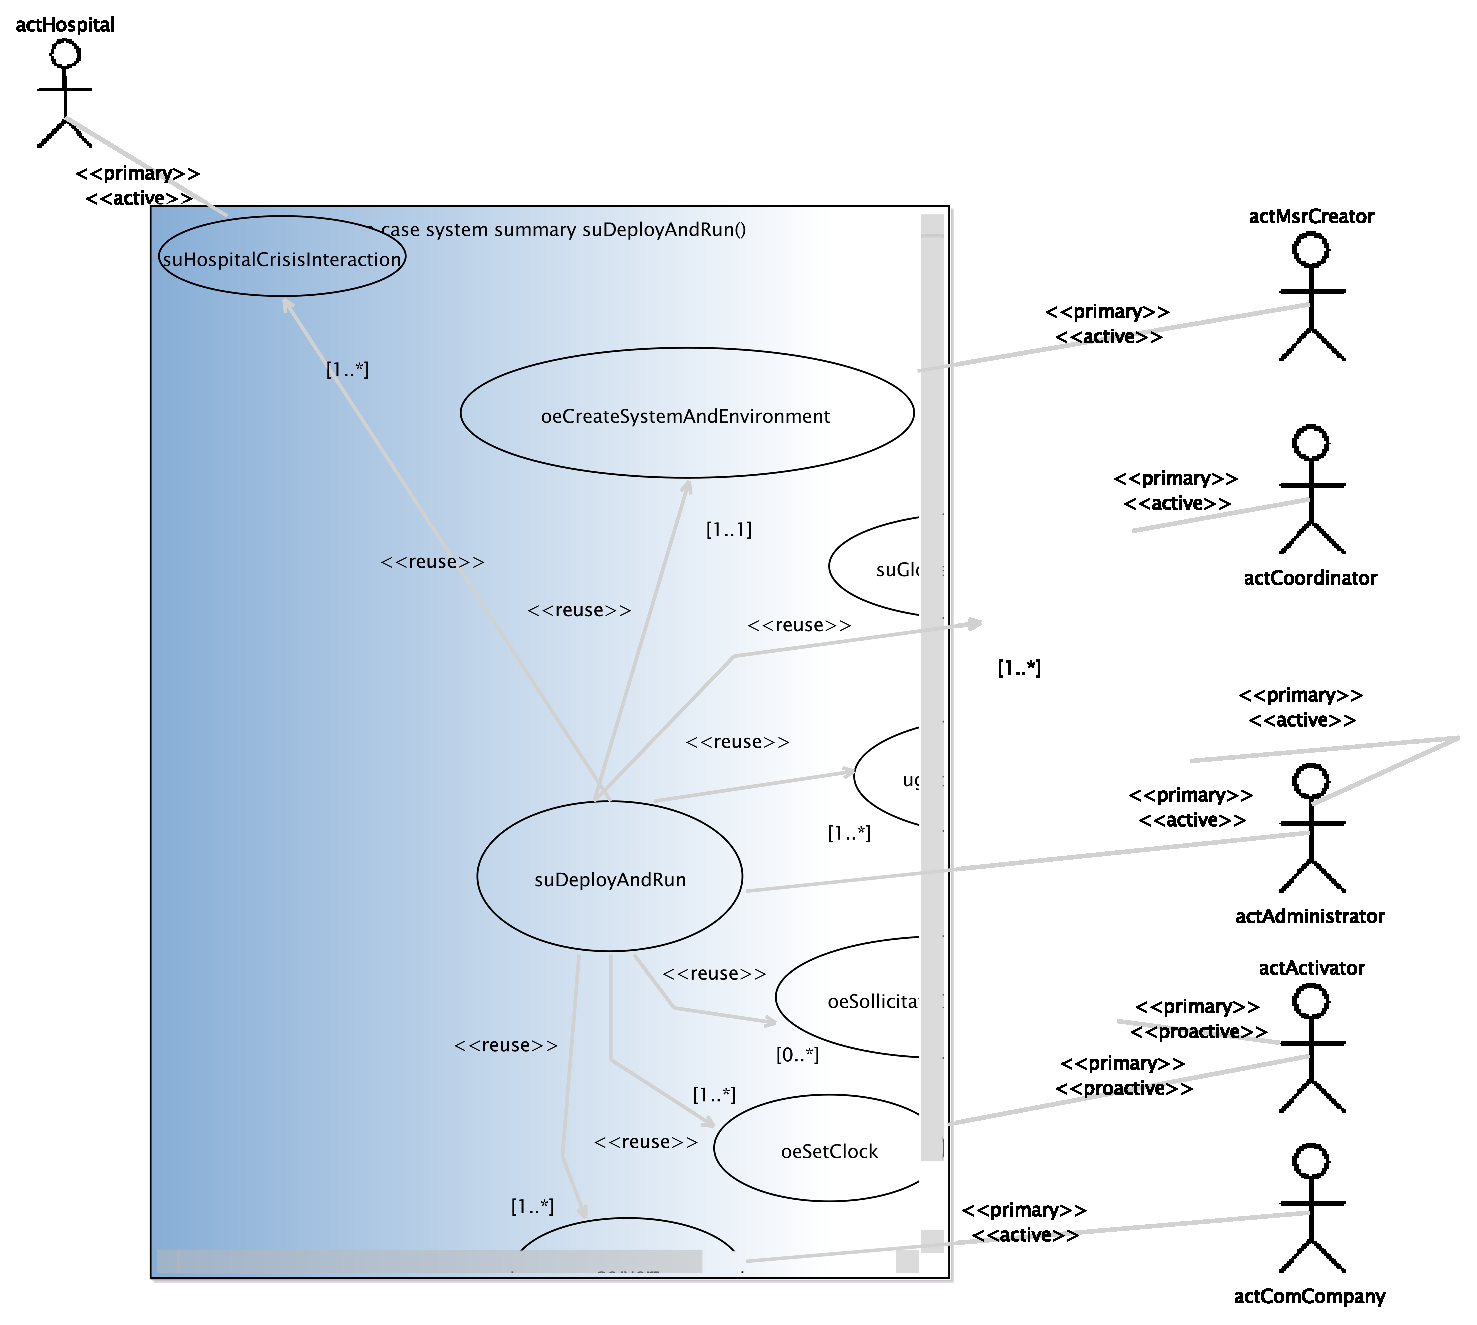
\includegraphics[
angle=0
,width=1.0\textwidth
]{./images-report-gen/usecase-model/summary/uc-suDeployAndRun.eps}
\end{center}
\caption[lu.uni.lassy.excalibur.examples.icrash Use Case Diagram: uc-suDeployAndRun]{ suDeployAndRun summary use case}
\label{fig:lu.uni.lassy.excalibur.examples.icrash-RE-UCD-uc-suDeployAndRun}
\end{figure}
\vspace{0.5cm}
